\documentclass[type=msc,nochapterpage,colorback,accentcolor=tud2c]{tudthesis}

%======================================================
% General package loading and definitions
%======================================================
\usepackage{inputenc} 
\usepackage{textcomp} 
\usepackage{ngerman}
\usepackage[american]{babel}
\usepackage{xspace}
\usepackage[fleqn]{amsmath} % math environments and more by the AMS 

\newcommand{\getmydate}{%
  \ifcase\month%
    \or Januar\or Februar\or M\"arz%
    \or April\or Mai\or Juni\or Juli%
    \or August\or September\or Oktober%
    \or November\or Dezember%
  \fi\ \number\year%
}

\begin{document}
  \thesistitle{Realizing Iterative Relaxed Scheduler in Kernel Space}%
    {}
  \author{Sreeram Sadasivam}
  \referee{Patrick Metzler}{Prof Neeraj Suri Ph.D}
  \department{Fachbereich Informatik}
  \group{DEEDS}
%  \dateofexam{\today}{\today}
  \makethesistitle
  \affidavit{Sreeram Sadasivam}

  \tableofcontents
  \listoffigures
  \listoftables
 
   \newpage

  
 
  \begin{abstract}
  \end{abstract}

  %*****************************************
  \chapter{Background}\label{ch:background} 
  %*****************************************
  \section{Software Verification}

Software programs are becoming increasingly complex. 
With the rise in complexity and technological advancements, components within a software have become susceptible to various erroneous conditions. 
Software verification have been perceived as a solution for the problems arising in the software development cycle. 
Software verification is primarily verifying if the specifications are met by the software~\citep{ghezzi2002fundamentals}.

There are two fundamental approaches used in software verification - dynamic and static software verification~\citep{ghezzi2002fundamentals}. 
Dynamic software verification is performed in conjunction with the execution of the software. 
In this approach, the behavior of the execution program is checked- commonly known as Test phase. 
Verification is succeeding phase also known as Review phase. 
In dynamic verification, the verification adheres to the concept of test and experimentation. 
The verification process handles the test and behavior of the program under different execution conditions. 
Static software verification is the complete opposite of the previous approach. 
The verification process is handled by checking the source code of the program before its execution. 
Static code analysis is one such technique which uses a similar approach. 

The verification of software can also be classified in perspective of automation - manual verification and automated verification. 
In manual verification, a reviewer manually verifies the software. 
Whereas in the latter approach, a script or a framework performs  verification. 

Software verification is a very broad area of research. 
This thesis work is focused on automated software verification for multithreaded programming. 

\section{Multithreaded Programming \label{multi_thread}}

Computing power has grown over the years. 
Advancements are made in the domain of computer architecture by moving the computing power from single-core to multi-core architecture. 
With such advancement, there were needs to adapt the programming designs from a serialized execution to more parallelizable execution. 
Various parallel programming models were perceived to accommodate the perceived progression. 
Multithreaded programming model was one of the designs considered for the performance boost in computing~\citep{carver2005modern}. 

Threads are small tasks executed by a scheduler of an operating system, where the resources such as the processor, TLB (Translation Lookaside Buffer), cache, etc., are shared between them. 
Threads share the same address space and resources. 
Multithreading addresses the concept of using multiple threads for having concurrent execution of a program on a single or multi-core architectures. 
Inter-thread communication is achieved by shared memory. 
Mapping the threads to the processor core is done by the operating system scheduler. 
Multithreading is only supported in operating systems which has multitasking feature. 

Advantages of using multithreading include: 
\begin{itemize}
\item	Fast Execution
\item	Better system utilization
\item	Simplified sharing  and communication
\item 	Improved responsiveness - Threads can overlap I/O and computation.
\item	Parallelization
\end{itemize}

Disadvantages:
\begin{itemize}
\item	Race conditions
\item	Deadlocks with improper use of locks/synchronization
\item	Cache misses when sharing memory
\end{itemize}

\section{Concurrency Bugs \label{con_bugs}}

Concurrency bugs are one of the major concerns in the domain of multithreaded environment. 
These bugs are very hard to find and reproduce. 
Most of these bugs are propagated from the mistakes made by the programmer~\citep{lopez2017study}. 
Some of these concurrency bugs include:
\begin{itemize}
\item	Data Race
\item 	Order violation
\item	Deadlock
\item	Livelock
\end{itemize}

Multithreaded programming yields non-deterministic execution order of a multithreaded program. 
Non-deterministic execution order indicates different executions order for the same multithreaded program. 
These different execution orders can generate different results. 
Thus, non-deterministic behavior of threads is one of the reasons for having the among mentioned bugs. 
Data race and order violation are classified as race condition bugs~\citep{lopez2017study}. 
Whereas, deadlock and livelock are classified as lack of progress bugs~\citep{lopez2017study}. 

\subsection{Race Condition}

Race condition is one of the most class of common concurrency problems.  
The problem arises, when there are concurrent reads and writes of a shared memory location. 
As stated above, the problem occurs with non-deterministic execution of threads. 

Consider the following example, you have three threads and they share two variables \emph{x} and \emph{y}~\citep{carver2005modern}. 
The value of \emph{x} is initially 0. 

\begin{table}[h]
\centering
\begin{tabular}{*{3}{c}}
Thread 1 & Thread 2 & Thread 3 \\
\hline
 (1) \emph{x} = 1 & (2) \emph{x} = 2 & (3) \emph{y} = \emph{x}\\
\end{tabular}
\caption{Race condition example}
\label{race_cond}
\end{table}

If the statements (1), (2) and (3) were executed as a sequential program. 
The value of \emph{y} would be 2. 
When the same program is split to three threads as shown in the above Table~\ref{race_cond}, the output of \emph{y} becomes unpredictable. 
The possible values of \emph{y} = \{0,1,2\}. 
The non-deterministic execution of the threads makes the output of \emph{y} non-deterministic. 
Table~\ref{poss_exec} depicts possible executions for the above multithreaded execution. 

\begin{table}[h]
\centering
\begin{tabular}{*{2}{c}}
Execution Order & Value of \emph{y} \\
\hline
 (3),(1),(2)& 0\\
 (3),(2),(1)& 0\\
 (2),(1),(3)& 1\\
 (1),(3),(2)& 1\\
 (1),(2),(3)& 2\\
 (2),(3),(1)& 2\\
\end{tabular}
\caption{Possible executions}
\label{poss_exec}
\end{table}

The above showcased problem is classified as a race condition bug. 
An ordered execution of reads and writes can fix the problem. 

\subsection{Lack Of Progress}

Lack of progress is another bug class observed in multithreaded programs. 
Some of the bugs under this class include deadlocks and livelocks. 

\subsubsection{Deadlocks}

A deadlock is a state in which each thread in the thread pool is waiting for some other thread to take action. 
In terms of the multithreaded programming environment, deadlocks occur when one thread waits on a resource locked by another thread, which in turn is waiting for another resource locked by another thread. 
If a thread is unable to change its state indefinitely because the resource requested by it are being held by another thread, then the entire system is said to be in deadlock~\citep{chaki2005concurrent}. 

%----Example Picture depicting deadlock---
\tikzstyle{thread} = [circle, minimum size=.5cm, text centered, draw=black, fill=white!30]
\tikzstyle{resource} = [rectangle, minimum width=1cm, minimum height=1cm, text centered, draw=black, fill=white!30]

\begin{figure}[h]
\centering
\begin{tikzpicture}[node distance=2cm]
%Resources
\node (R1) [resource] {R$_1$};
\node (R2) [resource,below of=R1] {R$_2$};

%Threads
\node (T1) [thread,below of=R1,xshift =-1.5cm,yshift=1cm] {T$_1$};
\node (T2) [thread,below of=R1,xshift =1.5cm,yshift=1cm] {T$_2$};

%Arrows
\draw [->,thick] (R1.west) -- (T1);
\draw [->,thick] (R2.east) -- (T2);
\draw [->,thick] (T1) -- (R2.west);
\draw [->,thick] (T2) -- (R1.east);

\end{tikzpicture}
\caption{Dead Lock Example}
\label{deadlock_example}
\end{figure}

In the example depicted in Fig~\ref{deadlock_example}, we have two threads T$_1$, T$_2$ and two resource instances R$_1$, R$_2$. 
Thread T$_1$ holds resource R$_1$ and waits for the acquisition of resource R$_2$ from thread T$_2$. 
Whereas T$_2$ cannot relinquish resource R$_2$, unless it acquires resource R$_1$ from T$_1$ for T$_2$'s progress. 
But resource R$_1$ is locked by T$_1$ which is waiting for R$_2$ from T$_2$. 
Thus, making a circular wait of resources. 
This example clearly explains the dependency of resources for the respective thread progress. 

A deadlock can occur if all the following conditions are met simultaneously.

\begin{itemize}
\item	Mutual exclusion
\item	Hold and wait
\item	No preemption
\item	Circular wait
\end{itemize}

These conditions are known as Coffman conditions~\citep{coffman_cond}.

Deadlock conditions can be avoided by scheduling the threads in a way to avoid the resource contention issue.

\subsubsection{Livelocks}

Livelocks are similar to deadlocks, except the state of threads change constantly but with none progressing. 
Livelocks are a special case of resource starvation of threads/processes. 
Some deadlock detection algorithms are susceptible to livelock conditions when more than one process/thread tries to take action~\citep{lopez2017study}\citep{chaki2005concurrent}. 
The above mentioned situation can be avoided by having one priority process/thread taking up the action. 

\section{Model Checking \label{model_check}}

From section~\ref{con_bugs}, it is very clear that there needs to be verification for multithreaded programs. 
The verification solutions range from detecting causality violations to correctness of execution~\citep{d2008survey}. 
Model checking is an example of such a technique. 
It is used for automatically verifying correctness properties of finite-state concurrent systems~\citep{model_check}\citep{berard2013systems}. 
This technique has a number of advantages over approaches that are based on simulation, testing and deductive reasoning. 
When solving a problem algorithmically, both the model of the system and the specification are formulated in a precise mathematical language. 
Finally, the problem is formulated as a task in logic, namely to verify whether a given structure adheres to a given logical formula.  
The technique has been successfully used in practice to verify complex sequential designs and communication protocols~\citep{model_check}. 
The model checker tries to verify all possible states of a system in a brute force manner~\citep{model_checking_principles}. 
Thus, making state space explosion as one of the major challenges.
In section~\ref{state_exp_prob}, we discuss more about the state explosion problem. 
Model checking tools usually verify the partial specification for liveness and safety properties~\citep{d2008survey}. 
Model checking tools generate a set of states from the instructions of a program, which are later analyzed. 
There is a need to store these states for asserting the number of visits made on them are at-most once. 
There are two methods commonly used to represent states:
\begin{itemize}
\item	Explicit-state model checking
\item	Symbolic model checking
\end{itemize}

%\paragraph{Advantages of using model checking:} 
%\begin{itemize}
%\item	Generic verification approach used across various domains of software engineering.
%\item 	Supports partial verification, more suited for assessment of essential requirements for a software.
%\item 	Not vulnerable to the likelihood that an error is exposed. 
%\item  	Provides diagnostic information thus, making it suitable for debugging purposes. 
%\item	Based on graph theory, data structures and logic thus, making it `sound and mathematical underpinning'. 
%\item 	Easy to understand and deploy. 
%
%\end{itemize}
%
%\paragraph{Disadvantages of using model checking:}
%\begin{itemize}
%\item	State explosion problem.
%\item	Appropriate for control-intensive applications rather than data-intensive applications. 
%\item	Verifies system model and not the actual system. 
%\item	Decidability issues when considering abstract data types or infinite state systems.
%\end{itemize}

\subsection{State explosion problem \label{state_exp_prob}}

The state space of a program is exponential in nature when it comes to number of variables, inputs, width of the data types, etc,. 
Presence of function calls and dynamic memory allocation makes it infinite~\citep{d2008survey}. 
Concurrency makes the situation worse by having interleaving of threads during execution. 
Interleaving generates exponential number of ways to execute a set of statements/instructions. 
Thus, having an explosion in state space. 
There are various techniques used to avoid the \emph{state explosion problem}. 
 
\subsection{Explicit-state Model Checking}

Explicit-state model checking methods recursively generate successors of initial state by constructing a state transition graph. 
Graphs are constructed using depth-first, breadth-first or heuristic algorithms. 
Erroneous states are determined `on the fly' thus, reducing the state space. 
A property violation on the newly generated states are regarded as erroneous states. 
Hash tables are used for indexing the explored states. 
If there is insufficient, memory lossy compression algorithms are used to accommodate the storage of hash tables~\citep{d2008survey}. 
Explicit-state techniques are more suited for error detection and handling concurrency. 

\subsection{Symbolic Model Checking}

Symbolic model checking methods manipulate a set of states rather than single states. 
Sets of states are represented by formulae in propositional logic. 
It can handle much larger designs with hundreds of state variables. 
Symbolic model checking uses different model checking algorithms: fix-point model checking(mainly for CTL), bounded model checking(mainly for LTL), invariant checking, etc,. 
Two main symbolic techniques used - Binary Decision Diagrams(BDD) and Propositional Satisfiability Checkers(SAT solvers). 
BDDs are traditionally used to represent boolean functions. 
A BDD is obtained from a Boolean decision tree by maximally sharing nodes and eliminating redundant nodes. 
However, BDDs grow very large. 
The issues in using finite automata for infinite sets are analogous. 
Symbolic representations such as propositional logic formulas are more memory efficient, at the cost of computation time. 
Symbolic techniques are suitable for proving correctness and handling state-space explosion due to program variables and data types.


\subsection{Partial Order Reduction}

Partial Order Reduction(POR) is a technique used for reducing the size of state space to be searched by a model checking algorithm~\citep{por10yrs}. 
This technique exploits the independence of concurrently executed events. 
Two events are independent of each other when executing them either order results in the same global state~\citep{model_check}. 
A common model for representing concurrent software is to realize it as an interleaving model. 
In an interleaving model, we have a single linear execution of the program arranged in an interleaved sequence. 
Concurrently executed events appear to be ordered arbitrarily to each other. 
Considering all interleaving sequences would lead to extremely large state space. 
Constructing the full state graph would make the fitting into the memory difficult. 
Therefore, a reduced state graph construction is used in this technique. 
 
POR exploits the commutativity of concurrently executed transitions, which would result in the same state. 
Fig ~\ref{commutativity_example} depicts the commutativity behavior. 
$S$, $S_1$, $S_2$ and $R$ are various states of a given program and $\alpha_1$, $\alpha_2$ represents various transitions. 
Consider two paths $P_1$ and $P_2$. 
$P_1 = S \rightarrow S_1 \rightarrow  R$ and $P_2 = S \rightarrow S_2 \rightarrow  R$. 
$P_1$ and $P_2$ reaches the same final state $R$. 
Thus, showing us that commutativity of transitions $\alpha_1$, $\alpha_2$ on the given example. 





%----Example Picture depicting deadlock---
\tikzstyle{state} = [circle, minimum size=1cm, text centered, draw=black, fill=white!30]

\begin{figure}[h]
\centering
\begin{tikzpicture}[node distance=1.5cm]

%Threads
\node (S) [state] {S};
\node (S1) [state,below of=S,xshift =-1.25cm] {S$_1$};
\node (S2) [state,below of=S,xshift =1.25cm] {S$_2$};
\node (R) [state,below of=S2,xshift =-1.25cm] {R};

%Arrows
\draw [->,thick] (S) to node [above] {$\alpha_1\ \ \ \ \ \ $} (S1);
\draw [->,thick] (S) to node [above] {$\ \ \ \ \ \ \alpha_2$} (S2);
\draw [->,thick] (S1) to node [below] {$\alpha_2\ \ \ \ \ \ $}  (R);
\draw [->,thick] (S2) to node [below] {$\ \ \ \ \ \ \alpha_1$}  (R);

\end{tikzpicture}
\caption{Commutativity Example}
\label{commutativity_example}
\end{figure}

Partial order reduction derives its motivation from the early versions of algorithms used for partial order modeling of program execution. 
POR is described as model checking using representatives~\citep{por_repr}. 
Verification is performed using representatives from equivalence classes of behaviors. 

The transitions of a system play a major role in the POR. 
POR is based on the dependency relation that exists between the transitions of a systems. 
A transition $\alpha \in T$ is enabled in a state $s$, if there is a state $s'$ such that $\alpha(s, s')$ holds. 
Otherwise, $\alpha$ is disabled in $s$. 
The set of transitions enabled in $s$ is $enabled(s)$. 
A transition $\alpha$ is deterministic, if for every state $s$ there is at most one state $s'$ such that $\alpha(s, s')$. 

A path $\pi$ from a state $s_0$ is a finite or infinite sequence. 

$\pi = s_0 \rightarrow s_1 \rightarrow ...$

$\alpha_0(s_0, s_1)$, $\alpha_1(s_1, s_2)$ are transitions on the states in path $\pi$ such that for every $i$, $\alpha_i(s_i, s_{i+1})$ holds. 
If $\pi$ is finite, then the length of $\pi$ is the number of transitions in $\pi$ and will be denoted by $\mid \pi \mid$. 
Purpose of POR is to reduce the number of states, while preserving the correctness of the program. 
A reduced state graph is generated using depth-first or breadth-first search methods. 
Model checking algorithm is applied to the resultant graph, which has fewer states and edges. 

An independence relation $I \subseteq T \times T$ is a symmetric, anti-reflexive relation such that for $s \in S$ and $(\alpha, \beta) \in I$:
\begin{itemize}
\item Enabledness 	If $\alpha,\beta \in enabled(s)$ then $\alpha \in enabled(\beta(s))$.
\item Commutativity	$\alpha, \beta \in enabled(s)$ then $\alpha(\beta(s)) = \beta(\alpha(s))$.
\end{itemize}
The dependency relation $D$ is the complement of $I$, namely $D = (T \times T) \setminus I$. The enabledness condition states that a pair of independent transitions do not disable one another. 
However, that it is possible for one to enable another. 
Stuttering refers to a sequence of identically labeled states along a path. 
In fig~\ref{commutativity_example}, we have two paths $P_1$ and $P_2$ which are stuttering equivalent. 
Thus, the reduced graph would have fewer number of states and retains the correctness property of the model. 

Two main POR techniques which are commonly considered: persistent/stubborn sets and sleep sets. 
Persistent set technique computes a provably-sufficient subset of the set of enabled transitions in each visited state such that unselected enabled transitions are guaranteed not to interfere with the execution of those being selected. 
The selected set is called a persistent set. 
Whereas, the most advanced algorithms are based on stubborn sets. 
These algorithms exploit information about ``which communication objects in a process gets committed to in a given set of operations in future''~\citep{dynamic_por}. 
Such an information is generally obtained from static code analysis. 
The sleep set technique exploits information on dependencies exclusively among transitions enabled in the current state along with information recorded about the past of the search. 
Both the techniques can be used simultaneously and are complementary. 
Unfortunately, existing persistent/stubborn set techniques suffer from a severe fundamental limitation in the context of concurrent software systems. 
The non-determinism in the execution of the concurrent programs makes the computation of precision difficult. 
Sleep sets could be used but, it cannot avoid state explosion. 
To overcome the above limitations, we have Dynamic POR, which is discussed further in the next section. 

\subsection{Dynamic POR}

Dynamic POR is a technique, which dynamically tracks interactions between processes and then exploits this information to identify back tracking points where alternative paths in the state space need to be explored~\citep{dynamic_por}. 
The algorithm works on depth first search in the reduced state space of the system. 
Dynamic POR helps to calculate dependencies dynamically during the exploration of the state space. 
It is able to adapt the exploration of the program's state graph to the precision of having another read or write operation accesses on the same memory location in the same execution path. 
The dynamic POR algorithm by \citet{dynamic_por} explores single transitions and performs recursive calls subsequently. 
A persistent set is calculated at each state in the state graph of a system.

\begin{figure}[h]
\centering
\subfloat [Traditional Mapping]{
\begin{tikzpicture}[ele/.style={fill=black,circle,minimum width=.8pt,inner sep=1pt},every fit/.style={ellipse,draw,inner sep=-2pt}]
  \node[ele,label=left:$a$] (a1) at (0,4) {};    
  \node[ele,label=left:$b$] (a2) at (0,3) {};    
  \node[ele,label=left:$c$] (a3) at (0,2) {};
  \node[ele,label=left:$d$] (a4) at (0,1) {};
  \node[above= of a1,anchor=south] {$Inputs$};	

  \node[ele,,label=right:$1$] (b1) at (4,4) {};
  \node[ele,,label=right:$2$] (b2) at (4,3) {};
  \node[ele,,label=right:$3$] (b3) at (4,2) {};
  \node[ele,,label=right:$4$] (b4) at (4,1) {};
  \node[above= of b1,anchor=south] {$Schedules$};	

  \node[draw,fit= (a1) (a2) (a3) (a4),minimum width=2cm] {} ;
  \node[draw,fit= (b1) (b2) (b3) (b4),minimum width=2cm] {} ;  
  \draw[->,thick,shorten <=2pt,shorten >=2pt] (a1) -- (b1);
  \draw[->,thick,shorten <=2pt,shorten >=2pt] (a1) -- (b2);
  \draw[->,thick,shorten <=2pt,shorten >=2pt] (a1) -- (b3);
  \draw[->,thick,shorten <=2pt,shorten >=2pt] (a1) -- (b4);
  \draw[->,thick,shorten <=2pt,shorten >=2] (a2) -- (b1);
  \draw[->,thick,shorten <=2pt,shorten >=2] (a2) -- (b2);
  \draw[->,thick,shorten <=2pt,shorten >=2] (a2) -- (b3);
  \draw[->,thick,shorten <=2pt,shorten >=2] (a2) -- (b4);
  \draw[->,thick,shorten <=2pt,shorten >=2] (a3) -- (b1);
  \draw[->,thick,shorten <=2pt,shorten >=2] (a3) -- (b2);
  \draw[->,thick,shorten <=2pt,shorten >=2] (a3) -- (b3);
  \draw[->,thick,shorten <=2pt,shorten >=2] (a3) -- (b4);
  \draw[->,thick,shorten <=2pt,shorten >=2] (a4) -- (b1);
  \draw[->,thick,shorten <=2pt,shorten >=2] (a4) -- (b2);
  \draw[->,thick,shorten <=2pt,shorten >=2] (a4) -- (b3);
  \draw[->,thick,shorten <=2pt,shorten >=2] (a4) -- (b4);
 \end{tikzpicture}\label{trad_map}}
 \subfloat[Deterministic Mapping]{
 \begin{tikzpicture}[ele/.style={fill=black,circle,minimum width=.8pt,inner sep=1pt},every fit/.style={ellipse,draw,inner sep=-2pt}]
  \node[ele,label=left:$a$] (a1) at (0,4) {};    
  \node[ele,label=left:$b$] (a2) at (0,3) {};    
  \node[ele,label=left:$c$] (a3) at (0,2) {};
  \node[ele,label=left:$d$] (a4) at (0,1) {};
  \node[above= of a1,anchor=south] {$Inputs$};	

  \node[ele,,label=right:$1$] (b1) at (4,4) {};
  \node[ele,,label=right:$2$] (b2) at (4,3) {};
  \node[ele,,label=right:$3$] (b3) at (4,2) {};
  \node[ele,,label=right:$4$] (b4) at (4,1) {};
  \node[above= of b1,anchor=south] {$Schedules$};	

  \node[draw,fit= (a1) (a2) (a3) (a4),minimum width=2cm] {} ;
  \node[draw,fit= (b1) (b2) (b3) (b4),minimum width=2cm] {} ;  
  \draw[->,thick,shorten <=2pt,shorten >=2pt] (a1) -- (b4);
  \draw[->,thick,shorten <=2pt,shorten >=2] (a2) -- (b2);
  \draw[->,thick,shorten <=2pt,shorten >=2] (a3) -- (b1);
  \draw[->,thick,shorten <=2pt,shorten >=2] (a4) -- (b3);
 \end{tikzpicture}\label{determinisitic_mapping}}
 \caption{Input to Schedule mappings in multithreaded execution based on the \citet{parrot}}
\end{figure}

\section{Deterministic Multi-Threading \label{sec_dmt}}

In sections \ref{multi_thread} and \ref{con_bugs}, we discussed about the non-determinism offered by multithreaded programming designs and the bugs associated with them. 
By adhering to a deterministic execution, a multithreaded program can avoid heisenbugs in the designs. 
In this section, we discuss about an approach which enforces deterministic execution to concurrent programs. 
The determinism in the execution of concurrent programs are achieved by enforcing scheduling constraints during shared memory events, synchronization operations or during lock acquisitions. 
Deterministic Multithreading(DMT) is a technique which addresses the above hypothesis. 

DMT solutions presents a design methodology of enforcing a single schedule or execution trace for a given input of the program as depicted in figure~\ref{determinisitic_mapping}. 
In the figure, we have set of inputs mapped to a set of schedules. 
Figure~ \ref{trad_map} depicts the non-deterministic execution of the same multithreaded program. 
Deterministic execution shown figure~\ref{determinisitic_mapping} can be achieved by determining points of synchronization or communication in the programs. 
Dthreads~\citep{dthreads}, KENDO~\citep{kendo} and GRACE~\citep{grace} presents a deterministic solution using synchronization points in the program as the execution point to enforce determinism. 
COREDET~\citep{coredet} presents solution based on memory level granularity. 
In COREDET, a deterministic round-robin scheduler is executed at the occurrence of a shared memory event. 
There are many frameworks - CoreDet~\citep{coredet}, Parrot~\citep{parrot}, Kendo~\citep{kendo}, DThreads~\citep{dthreads}, Grace~\citep{grace}, which adheres to this principle. 
Some of these frameworks are discussed further in the next chapter. 

DMT solutions can be observed as a solution from the area of concurrency testing because they help to reduce the number of necessary test cases in the multithreaded program. 
These solutions trade potential execution time overhead(overhead in regard with execution of unmodified program) by reducing the non-determinism in multithreaded program for simplifying the testing process. 
DMT solutions do not control the schedule in advance, thus making them unsuitable for automated verification of concurrent programs. 
Moreover, it is not possible to adjust the level of non-determinism in these solutions. 
Migrating these DMT solutions to perform program verification is unrealistic because, their scheduling constraints depend on concrete program inputs which, would require to verify all possible inputs separately. 
DMT solutions provides fixed scheduling constraints and cannot be relaxed during runtime~\citep{metzler2017quick}. 
They also do not provide any fairness in scheduling or for parts of the program by completely unconstrained scheduling. 



\begin{figure}[h]
     \centering
     \subfloat[][Conventional Verification]{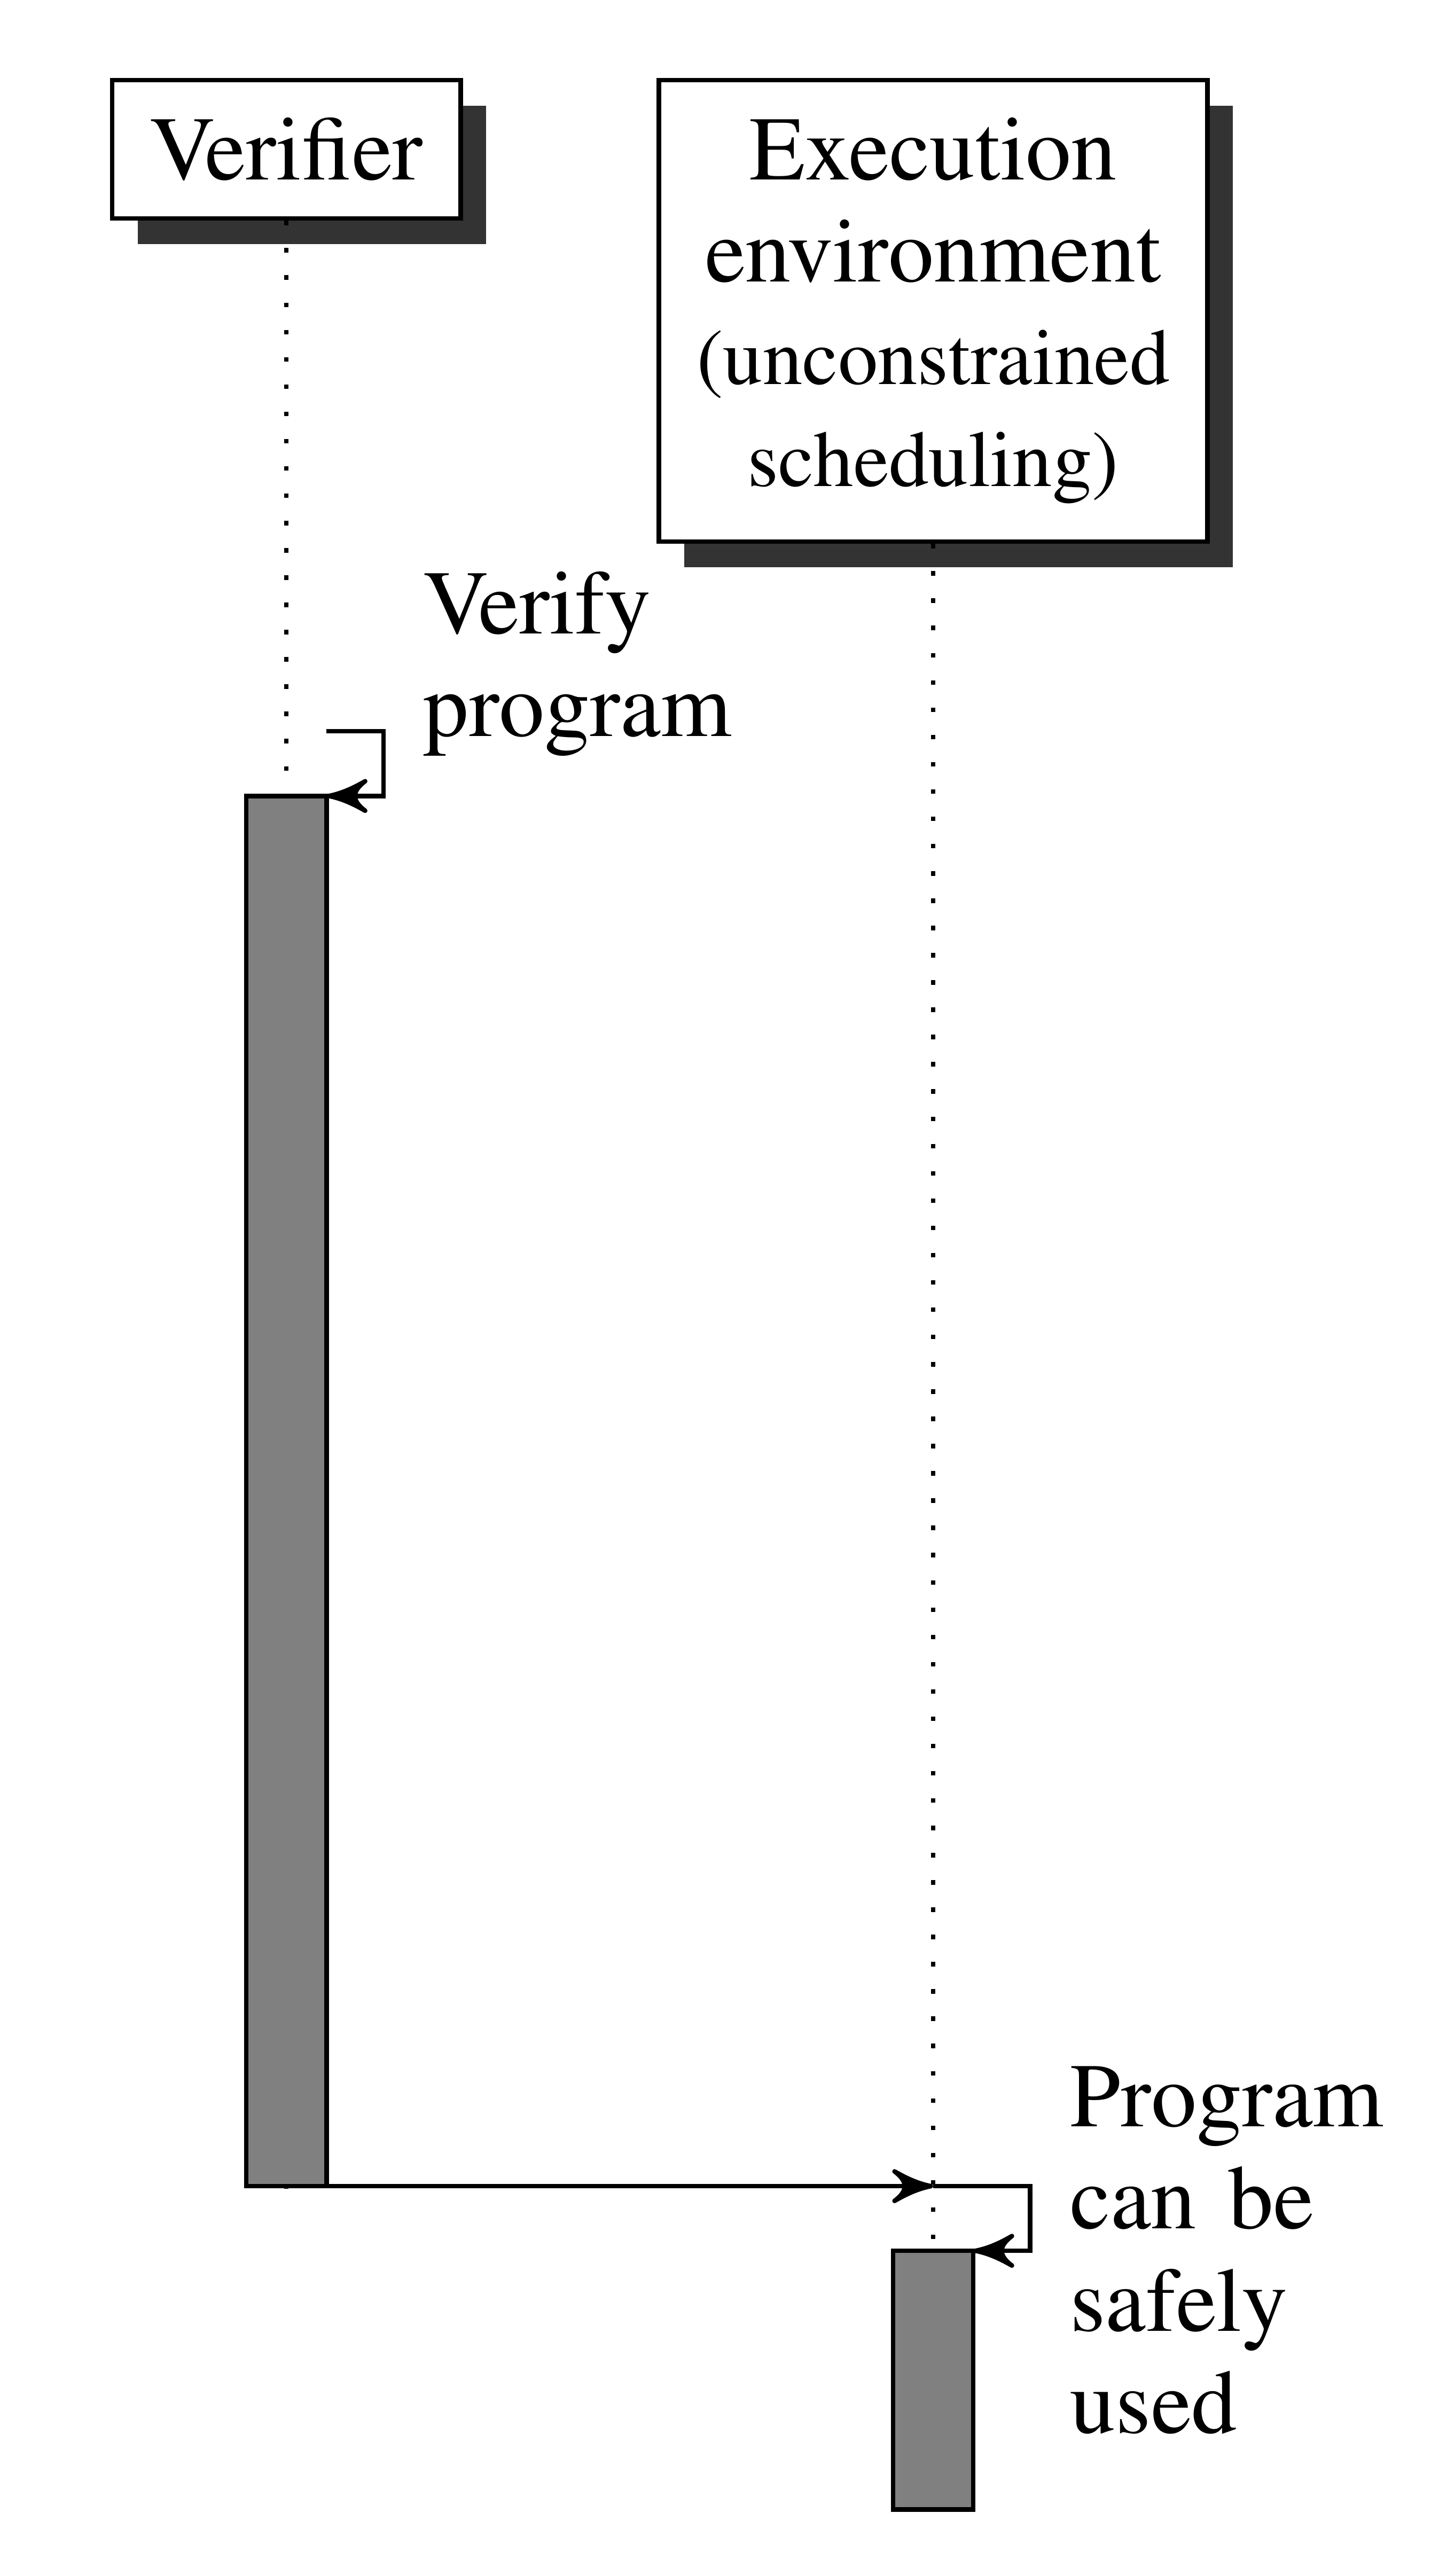
\includegraphics[scale=0.08]{figs/conventional.png}\label{conv_ver}}
     \subfloat[][Iterative Relaxed Scheduling]{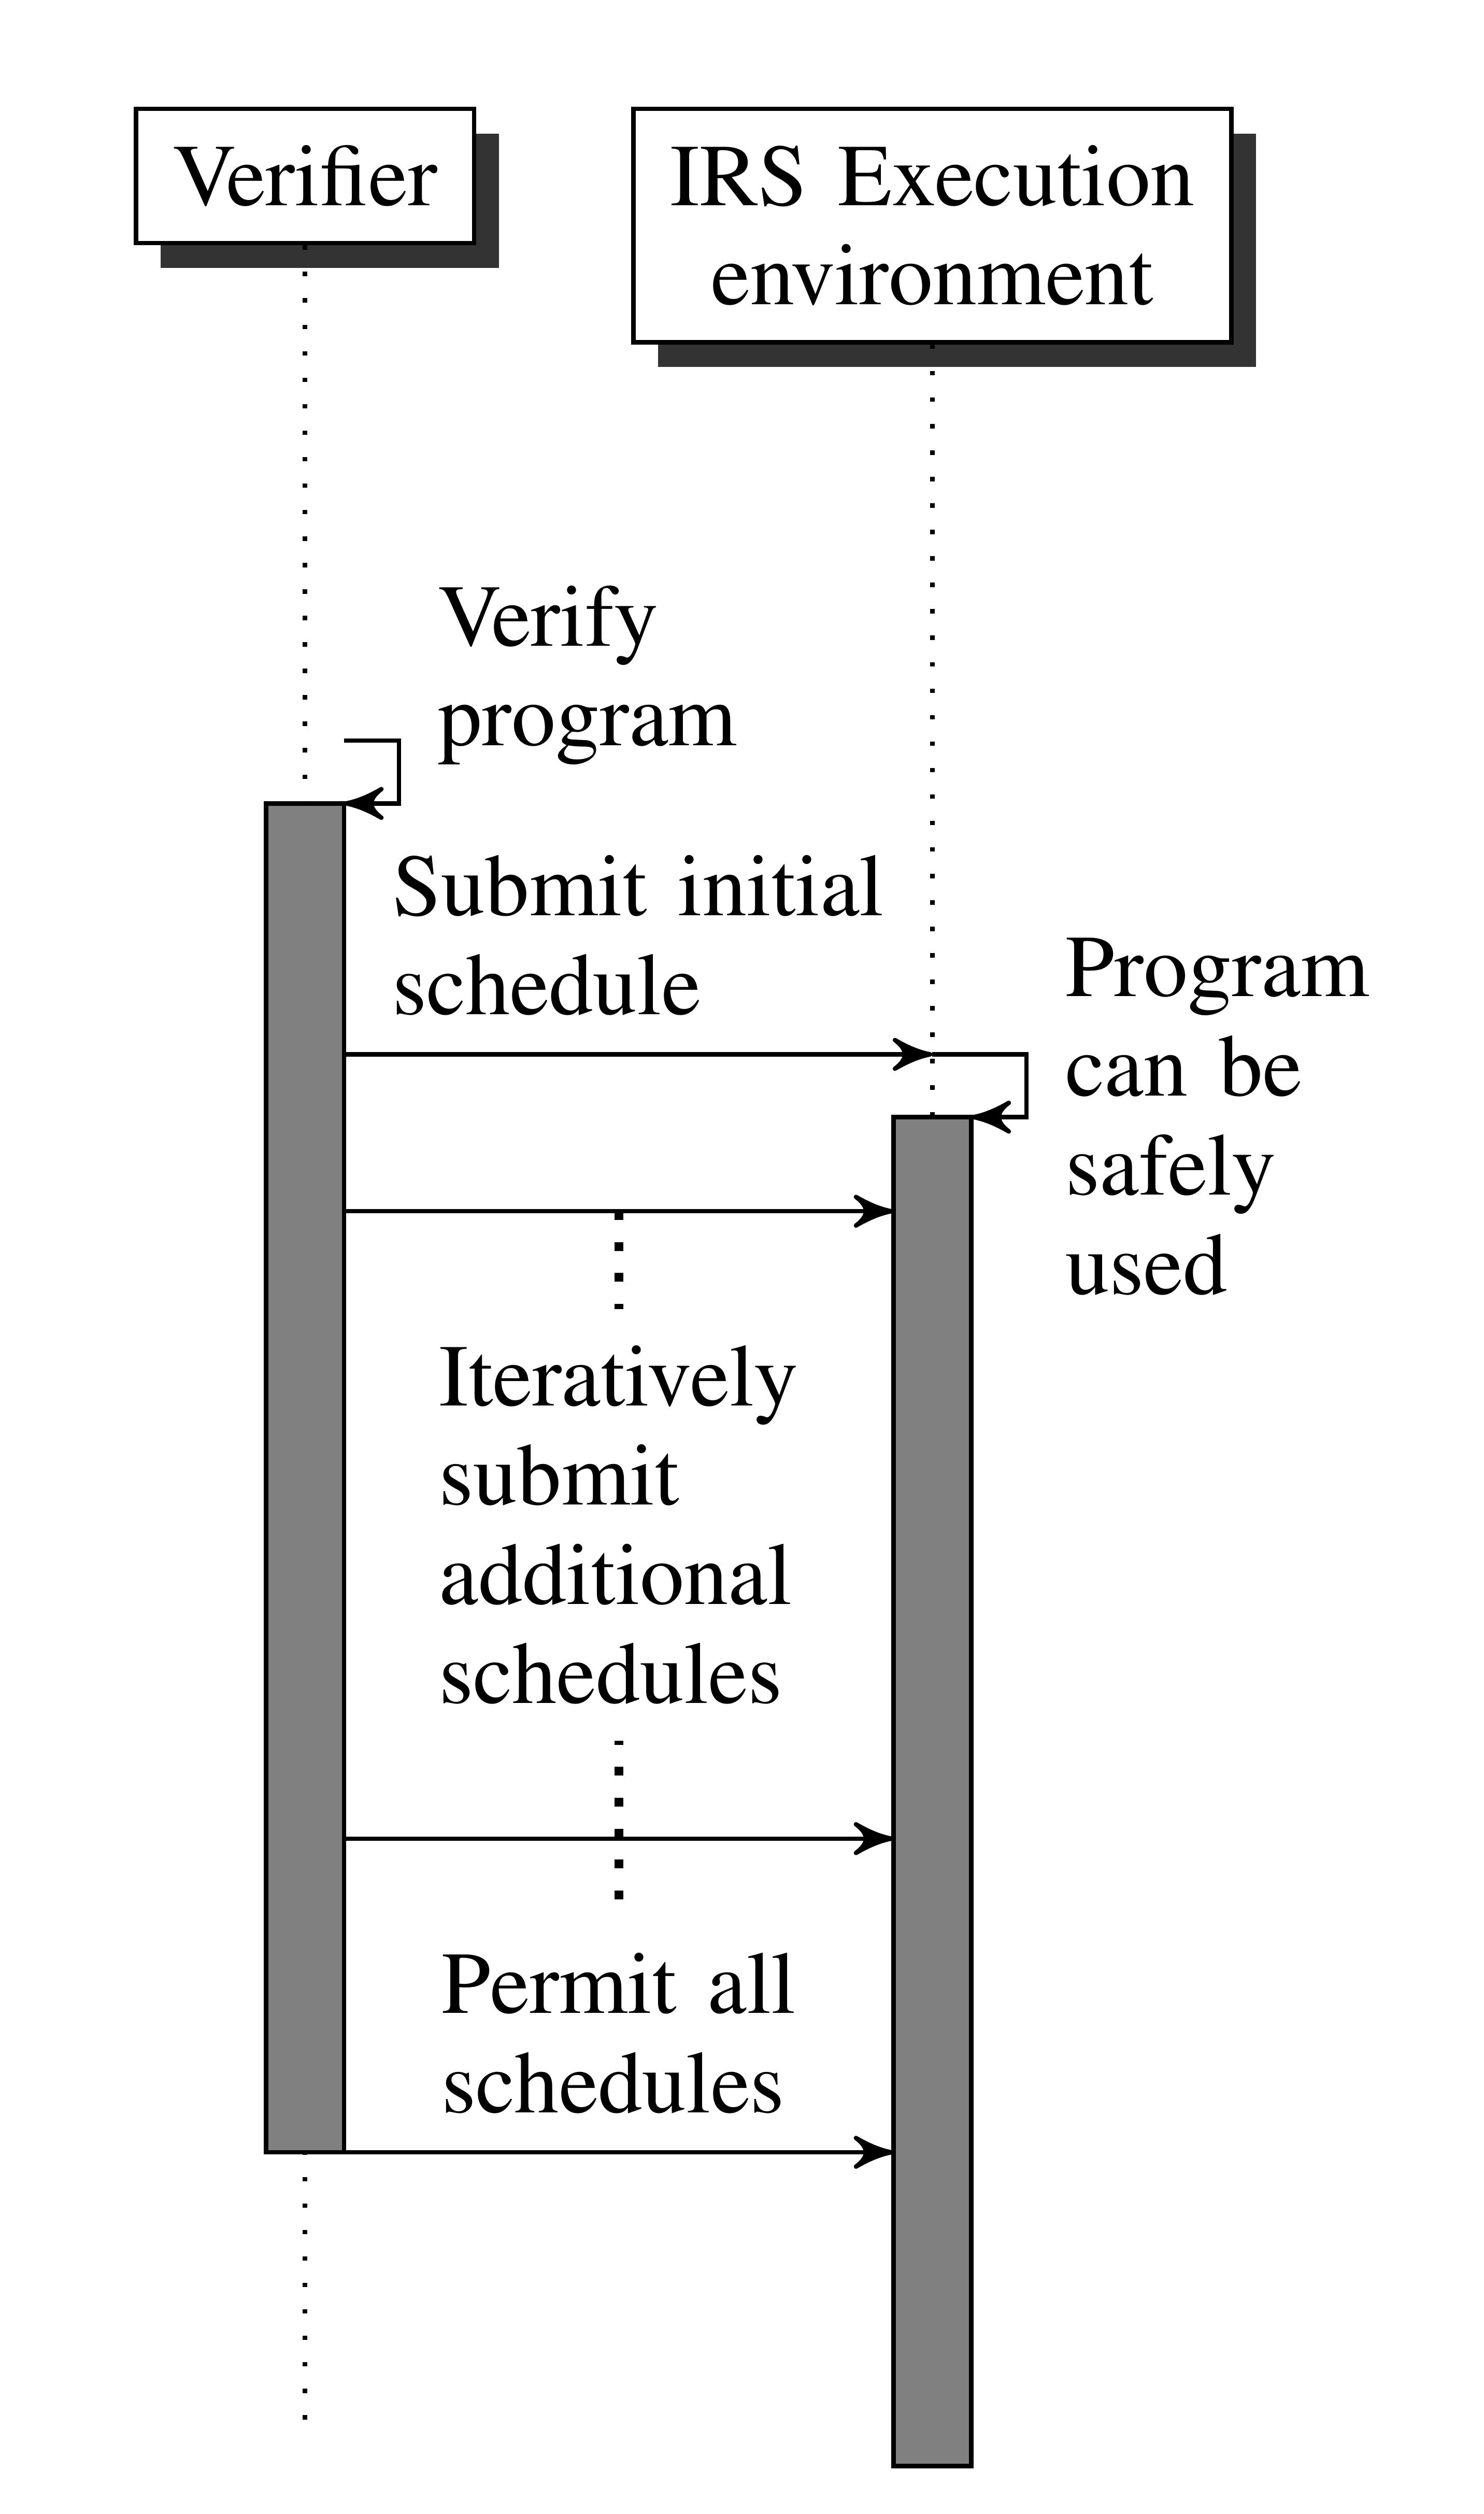
\includegraphics[scale=0.08]{figs/irs_only.png}\label{irs_only}}
     \caption{Conventional vs IRS verification adapted from \citet{metzler2017quick}}
\end{figure}


\section{Iterative Relaxed Scheduling \label{iter_rel_sched}}

From the previous section, it is abundantly clear the drawbacks of using DMT approaches for concurrency verification. 
Iterative relaxed scheduling(IRS) is a program verification technique used for concurrent programs. 
Figure~\ref{conv_ver} presents a conventional software verification approach for concurrent programs. 
The main drawback with such a verification technique is that it presents a huge verification delay. 
Large verification delay is presented from the non-deterministic nature of multithreaded programs. 
Software verification for concurrent programs presents large state spaces thus, leading to state-space explosion problem as discussed in section~\ref{state_exp_prob}. 
POR technique helps to reduce the state space problem by identifying the equivalence classes of program executions such that only one representative of each class needs to be verified. 
Mazurkiewicz trace~\citep{mazurkiewicz1986trace} is one such equivalence class representation. 
Verification delays would reach higher values for benchmark programs even if state-of-the-art POR is used~\citep{abdulla2014optimal}\citep{gueta2007cartesian}. 
The high complexity of state space exploration for concurrent systems is still a concern for large industrial software deployments. 
However, individual traces can be verified swiftly as observed when relating verification time to the number of explored traces. 
From DMT techniques we were able to conjure the reduction in the number of test cases. 
DMT solutions do not allow to control the schedule that will occur in advance, which makes them unsuitable for automated verification of multithreaded programs. 
In chapter~\ref{rel_work}, we discuss about the various DMT techniques in more detail and how it compares with the IRS solution. 

\citet{metzler2017quick} presents a novel implementation of software verification approach for concurrent programs through a new technique - iterative relaxed scheduling(IRS). 
IRS provides a way to adjust the amount of non-determinism thus, providing an adjustable verification delay in the system. 
In IRS instead of waiting for the entire verification to complete, we can use the intermediate verification results that guarantee program correctness with one or more schedules for the execution of the multithreaded program. 
Mazurkiewicz traces helps to use POR as a verification technique with intermediate verification results. 
Figure~\ref{irs_only} depicts the idea of IRS. 
IRS is in a way ``recorder-replay design''. 
The verifier in IRS submits intermediate schedules for IRS environment to execute which is similar to the ``recorder'' in ``recorder-replay'' designs. 
The scheduler in the IRS environment reuse the execution traces submitted by the verifier thus, making it ``replayer''. 
In chapter~\ref{rel_work}, we discuss some DMT solutions which use a similar design paradigm.  
IRS uses LLVM for instrumenting multithreaded programs which use shared memory design. 
The annotations in the instrumented program are in reference to the shared memory events within the program. 
Thus, IRS is able to provide fine grained memory level granularity. 
Mazurkiewicz traces generated by the verifier is obtained in relation with the shared memory events occuring in the mulithreaded program. 
With the scheduler and the recorded traces, IRS is able to enforce scheduling constraints to the multithreaded program. 

The IRS framework presented by \citet{metzler2017quick} uses two different design variants to realize the scheduler implementation. 
The IRS scheduler is realized entirely in the userspace. 
In this thesis, we present an alternative by moving the IRS scheduler to the kernel space. 
Chapter \ref{approach_ch} highlights the need for such migration and later discusses about the kernel space adaptation. 



  

  %*****************************************
  \chapter{Related Work}\label{ch:related_work} 
  %*****************************************
  The previous chapter highlighted the need for debugging tools or methodologies for solving concurrency bugs in multithreaded programming. 
This thesis is conceived with a solution based on iterative relaxed scheduling(IRS). 
However, there are other techniques which address various solutions using deterministic multithreading(DMT). 
In this chapter, we explore various DMT based solutions and the similarities they share with IRS. 

\section{DTHREADS}

\citet{dthreads} presents a deterministic multithreading runtime system. 
It is build on top of PThreads(POSIX Thread) library in Linux. 
The dthreads library replaces most of the pthread library functions with its own implementation enforcing determinism in execution of threads. 
All the threads created using dthreads library are created as processes and they use a deterministic memory commit protocol for synchronizing the conceived shared memory state. 
The idea of using ``threads-as-processes'' paradigm is motivated from the work of \citet{grace}. 
By moving the design to processes, dthreads eliminates false sharing and provides protection faults. 
For simplicity we would call these threads as dthreads. 
``Twining and diffing'' technique is used to perform the deterministic  memory commit protocol in dthreads. 
Dthreads are run independently until they reach a synchronization point where the diffing step of the above technique takes place. 
It compares the modification in the memory page with the twin page with contains the shared state. 
Each dthread enters the differential comparison(diffing) step based on token being passed around the dthreads. 
Dthreads consists of two phases of execution: parallel and serial phases. 
The twining-diffing step occurs in the serial phase of execution. 
Transitions to serial phase occurs statically. 
Any synchronization operation will result in a transition to serial phase. 

Dthreads creates private, per-process copies of modified pages between commits. 
This would increase the program's memory footprint by the number of modified pages between synchronization operations. 
In case of IRS, we have do not change the implementation of pthreads. 
Therefore, the above problem never occurs in IRS however, there is a possibility of false sharing. 
IRS implementation emphasizes on memory level granularity whereas, dthreads focuses on the synchronization operations encountered in the user program. 
IRS follows a recorder-replay model whereas, dthreads uses ``Twining and diffing'' of threads. 
In IRS, we have a verifier which records the execution traces that are deemed to be safe considering the correctness of the program execution. 
It also consists of a scheduler which can be considered as the replay part of the model. 
In this thesis, we migrate the scheduler module to the kernel space from user space. 
The scheduler would run the instrumented user program with the execution traces generated by the verifier. 
Dthreads does not have a verifier or a separate scheduler module instead, it has library level support to enforce the determinism in execution. 
Also it does not instrument the user program. 
Dthreads is C/C++ library support implemented entirely in user space whereas, in this thesis we highlight the IRS scheduler implemented in kernel space. 

\section{GRACE}

\citet{grace} presents a deterministic library support in Grace. 
The design is similar to the Dthreads implementation. 
Grace also uses ``threads-as-processes'' paradigm. 
However, it is primarily targeted at fork-join models. 
Grace focuses on multithreaded designs which highlight thread creation and joining. 
The reason for the inclusion is that it also falls under the category of DMT based solutions.
However, it has lot drawbacks - it focuses on fork-join models only. 
It is similar to dthreads in a lot of regard.  
IRS is completely different to the Grace implementation.

\section{PEREGRINE}

\citet{peregrine} conceives an alternative DMT solution with schedule relaxation in PEREGRINE runtime system. 
It is a record-replay based implementation. 
It combines two different scheduling designs - sync schedule and memory schedules. 
The hybrid scheduling design is enforce efficiency and determinism in the execution of multithreaded program. 
Unlike the previously mentioned DMT solutions, PEREGRINE uses an instrumentor in LLVM and a user space scheduler for the replay of execution trace. 
PEREGRINE executes the multithreaded program with a certain input to generate its execution trace. 
The recorder records the trace for the given input of the program. 
Replayer/scheduler reuses the same execution trace for the given input of the program. 
It enforces the execution trace on the user program for same input thus, providing a level of determinism in its execution. 
It shares a lot of similarities with IRS. 
IRS is also record-replay based design. 
Both these designs provide memory level granularity. 
However, IRS design generates more traces with less memory level constraints for iteration therefore, retaining some level of non-determinism in the execution of the program. 
The memory level determinism in IRS is enforced based on the order of the memory access. Whereas, in case of PEREGRINE it is enforced based on the output of the program. 
PEREGRINE uses the same execution trace for different inputs to the multithreaded program. 
Whereas, IRS improves the degree of non-determinism in the execution of multithreaded program with every iteration of verifier.

\section{KENDO}

KENDO is another DMT solution proposed by \citet{kendo}, which uses modified Linux kernel to support deterministic logical time. 
KENDO is a software framework, which enforces weak deterministic execution of general purpose lock-based C/C++ based multithreaded programs.  
Weak determinism ensures a deterministic order of all lock acquisitions for a given program input.   
KENDO is a subset of pthreads library. 
It achieves determinism with the use of deterministic logical time, which is used to track the progress of each thread in a deterministic manner. 
KENDO has a kernel level implementation to enforce deterministic execution of threads. 
The IRS implementation highlighted in this thesis focuses on a scheduler implemented in kernel space for enforcing the memory constraints provided in the execution traces by the verifier. 
KENDO does not have any instrumentation of user program unlike PEREGRINE or IRS. 
KENDO only focuses on determinism in lock acquisitions and not on all shared memory accesses whereas, IRS addresses memory-level granularity for all shared memory accesses in the multithreaded program.

\section{COREDET}

\citet{coredet} came up with a compiler and runtime system enforcing deterministic multithreaded execution in COREDET. 
It is another runtime implementation based on DMT. 
COREDET has two phases - parallel and serial phases similar to the Dthreads. 
It has an instrumentor tool in LLVM for instrumenting memory events similar to PEREGRINE. 
COREDET is one of the first DMT solution which addressed the shared memory events and provided memory level granularity. 
COREDET can be executed in two different ways - ownership tracking and store buffering. 
First approach tracks the ownership of data and serializes the execution whenever threads communicate. Such an approach yields sequentially consistent executions and lower overheads, but lower scalability. 
Second approach uses memory versioning without any form of speculation and relaxes memory ordering, yielding higher scalability at the cost of higher overheads.  
It shares a lot of similarities with IRS implementation. 
Both the solutions use LLVM for instrumenting memory events in the multithreaded program. 
However, COREDET uses a round-robin scheduling when it enters a serial phase of execution. 
Whereas in case of IRS on occurrence of a memory event, the scheduler checks for the memory access permission for the given thread with the recorded trace. 
COREDET does not have any record-replay implementation. 
It can be conceived as a runtime implementation with emphasis on fine grained memory access with serialized commits.  


\section{PARROT}

PARROT is another runtime solution based on DMT from \citet{parrot}. 
Compared to other DMT solutions which maps one schedule for one input as depicted in figure~\ref{determinisitic_mapping}, PARROT proposes an approach which uses stable multithreading(StableMT). 
In StableMT, we reuse each schedule on a wide range of inputs, mapping all inputs to a dramatically reduced set of schedules. 
PARROT is a pthread compactible implementation. 
PARROT provides weak determinism similar to KENDO but offers stability. 
PARROT can be integrated with DBUG\citep{dbug} - open source model checker in Linux for determining bugs in the schedules. 
\citet{parrot} shows us that PARROT-DBUG ecosystem is more effective than either system alone. 
DBUG checks the schedules that matter to PARROT and the developers. 
Whereas, PARROT reduces the number of schedules to be checked by DBUG thus, increasing the coverage of DBUG. 
Compared to IRS, PARROT does not have any static code analysis done inside the multithreaded programs. 
The determinism provided by PARROT is relative to three factors: external input, performance critical sections, data races with respect to the enforced synchronization schedules. 
IRS focuses on memory level granularity whereas, PARROT is focused on weak determinism similar to KENDO. 
PARROT-DBUG focuses on StableMT with exhaustive testing of all schedules whereas in IRS, the execution of a multithreaded program can be initiated with a single execution trace from the verifier. 
IRS generates a new trace for every iteration whereas in case of PARROT-DBUG, the execution is blocked until the DBUG checks all the schedules.

\section*{Inference}

From the above sections, it is abundantly clear that there not any solutions which come close to the IRS. 
COREDET is the only implementation which seems to provide memory level granularity similar to IRS. 
PEREGRINE is another implementation which depicts a record-replay paradigm similar to IRS. 
PARROT-DBUG presents a StableMT focused on checking a set of reduced schedules for all the provided inputs in the multithreaded program. 
Other solutions presented in this chapter focus on DMT solutions aimed at synchronization operations rather than memory level accesses. 

 


%  \bibiliography{thesis.bib}


  %\chapter{Generelle Informationen}
    %Die Klasse basiert auf der \textaccent{tudreport}-Klasse von C. v. Loewenich und
    %J. Werner. Alle "Anderungen dort wirken sich direkt auf die
    %\textaccent{tudthesis}-Klasse aus. Genauer: die \textaccent{tudthesis}-Klasse definiert nur einige
    %neue Befehle und legt die Formatierung der ersten zwei Seiten (Titelseite
    %und R"uckseite des Titleblattes) fest.

%\chapter{Verwendung der Klasse}
 % Die Klasse wird verwendet, indem in der Dokumentenpr"aambel
  %\textaccent{\textbackslash documentclass\{tudthesis\}}
  %eingetragen wird.

  
%\section{Klassenoptionen}
    %Die Klasse unterst"utzt alle Klassenoptionen der tudreport-Klasse.
    
%\paragraph{Neue Optionen}
    %\begin{itemize}
      %\item \textbf{type=<dr|drfinal|diplom|msc|pp|bsc|sta>}\\
        %Hiermit wird die Art der Arbeit angegeben. Dies legt verschiedene
        %Formatierungen fest.\\
        %\begin{tabular}{ll}
        %\textaccent{dr} &f"ur eingereichte Dissertationen\\
        %\textaccent{drfinal} &f"ur genehmigte Dissertationen\\
        %\textaccent{diplom} &f"ur Diplomarbeiten\\
        %\textaccent{msc} &f"ur Master-Theses\\
        %\textaccent{pp} &f"ur Project-Proposals\\
        %\textaccent{bsc} &f"ur Bachelor-Theses\\
        %\textaccent{sta} &f"ur Studienarbeiten
        %\end{tabular}
    %\end{itemize}

  %\section{Befehle}
   % \begin{itemize}\itemsep-0.5\parsep
    %  \item \textbf{\textbackslash thesistitle\{\#1\}\{\#2\}}\\
     %   \#1: Titel der Arbeit in der Erstsprache (z.B. Deutsch)\\
      %  \#2: Titel der Arbeit in der zweiten Sprache (z.B. Englisch)
      %\item \textbf{\textbackslash makethesistitle}\\
      %  Erzeugt die korrekte Titelseite
      %\item \textbf{\textbackslash author\{\#1\}}\\
      %  \#1: Name des Autors, bei Dr.-Arbeit zus"atzlich auch Geburtsort!
      %\item \textbf{\textbackslash date\{\#1\}}\\
       % Standard ist der aktuelle Monat und das aktuelle Jahr (z.B. \getmydate)\\
        %\#1: individuelles Datum
      %\item \textbf{\textbackslash referee\{\#1\}\{\#2\}[\#3]}\\
       % Namen der Gutachter, (3. Gutachter optional)
      %\item \textbf{\textbackslash department\{\#1\}}\\
       % Fachbereich an dem die Arbeit durchgef"uhrt wurde. Standard ist
        %\glqq Fachbereich Physik\grqq.
      %\item \textbf{\textbackslash group\{\#1\}}\\
       
% Arbeitsgruppe / Institut an dem die Arbeit durchgef"uhrt wurde
 %     \item \textbf{\textbackslash dateofexam\{\#1\}\{\#2\}}\\
  %      \#1: Tag der Einreichung der Arbeit\\
   %     \#2: Tag der Pr"ufung / Tag des Abschlusses\\
    %    \textaccentcolor{Wird nur bei \textaccent{type=drfinal} verwendet.
     %   Ansonsten wird ein leeres Feld erzeugt, in das bei Abgabe der 
      %  Arbeit ein Stempel gesetzt wird.}
      %\item  \textbf{\textbackslash affidavit[\#1]\{\#2\}}\\
       % \#1: Datum der Eigenst"andigkeitserkl"arung (optional)\\
        %\#2: Signatur unter der Unterschrift\\
  %  \end{itemize}

\end{document}
